%!TEX root = <main.tex>
\section{Optimizations}

In this section we explain \textit{incremental inference} and the two \textit{approximate inference} approaches, patch \textit{propagation thresholding} and \textit{adaptive drill-down}, in detail.
In \system~ these optimizations are applied on top of the current dominant approach of performing CNN inference on batches of images where each image corresponds to an occluded instance of the original image.
Batched inference is important as it reduces per image inference time by amortizing the fixed overheads.
In our experiments we found that this simple optimization alone can give up to ~1.4X speedups on CPU environments and ~2X speedups on the GPU environment compared to the per image inference approach.
Finally we explain how \system~ configures it's internal system configurations for \textit{approximate inference} by using a sample image set during the initial tuning stage.

\subsection{Incremental Inference}\label{sec:inc_computation}

As explained earlier, occlusion experiments in it's naive form performs many redundant computations.
In order to avoid these redundancies, layers in a CNN has to be change aware and operate in an incremental manner i.e. reuse previous computations as much as possible and compute only the required ones.
In this section we focus on transformations that operate on a local spatial context (i.e. Convolution and Pooling) as other types either has no redundancies (global context transformations) or is trivial to make incremental (point transformations).
The choice of CPUs vs GPUs for CNN inference also brings up new considerations for the batched implementation of these incremental transformations and we explain two version of implementations, one which is a naive implementation of batched incremental inference approach and the other a GPU optimized version.
We also explain incremental implementations of two other linear algebra operators, element-wise addition and depth-wise concatenation.

\vspace{2mm}
\noindent \textbf{Incremental Convolution and Pooling.}


\begin{table}[t]
  \centering
  \caption{Additional symbols used in the Optimizations Section}
  \scalebox{0.8}{\begin{tabular}{p{2cm}p{7.5cm}}
    \toprule
    \textbf{Symbol} & \textbf{Meaning}\\
    \midrule \midrule
    $x^I_P,y^I_P$ & Starting coordinates of the input patch\\
    \midrule
    $x^R_P,y^R_P$ & Starting coordinates of the patch that needs to be read in for the transformation\\
    \midrule
    $x^O_P,y^O_P$ & Starting coordinates of the output patch\\
    \midrule
    $H^I_P,W^I_P$ & Height, and width of the input patch\\
   	\midrule
   	$H^R_P,W^R_P$ & Height, and width of the patch that needs to be read in for the transformation\\
   	\midrule
   	$H^O_P,W^O_P$ & Height, and width of the output patch\\
    \midrule
    $\tau$ & Projective field threshold\\
    \bottomrule
  \end{tabular}}
\label{table:optimizer_symbols}
\end{table}


\begin{figure}[t]
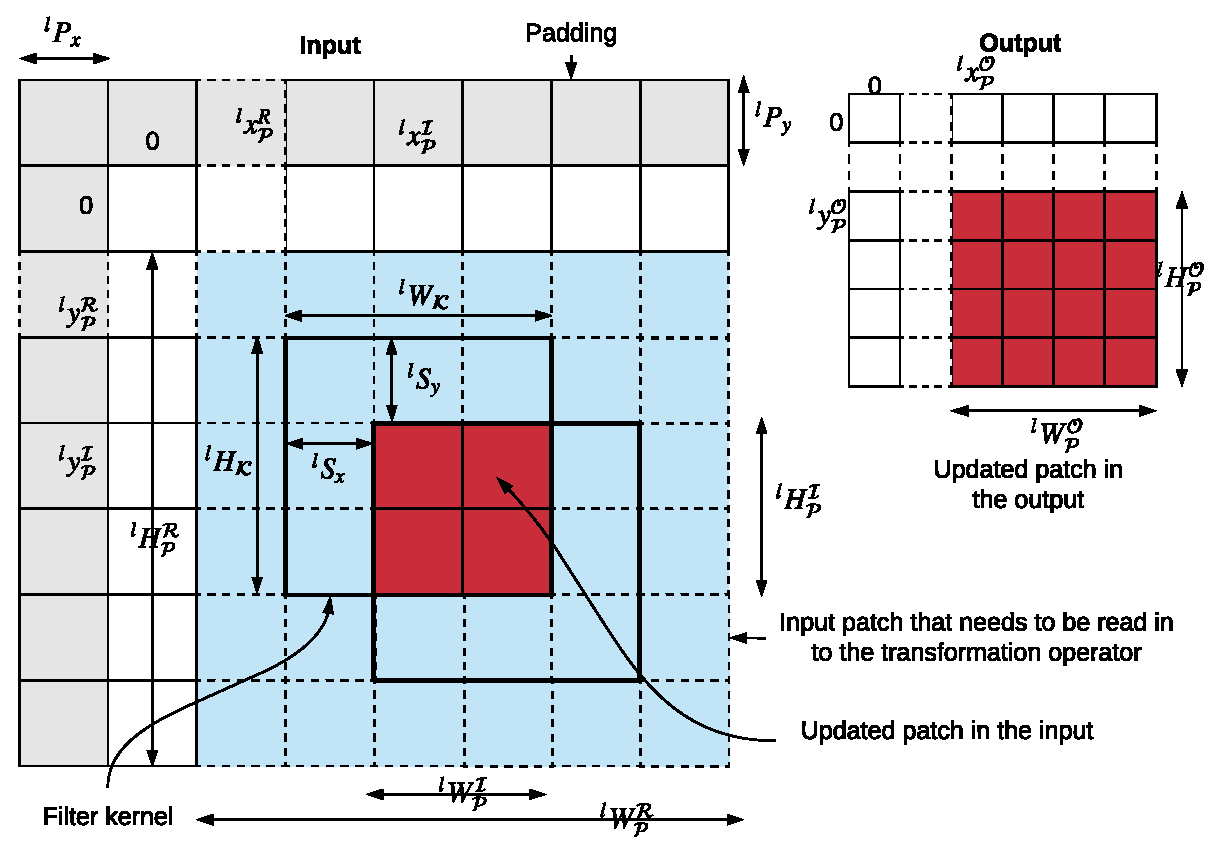
\includegraphics[width=\columnwidth]{images/dimensions}
\caption{Simplified representation of input and output patch coordinates and dimensions of Conv. and Pool transformations.}
\label{fig:dimensions}
\end{figure}

The two types of transformations in a CNN that operate on a local spatial context are Convolution and Polling. In Section \ref{sec:preliminaries} we showed that both of these transformations can be cast into a form of applying a filter along the spatial dimensions of the input volume.
However how each transformation operate along the depth dimension is different.
For our purpose we are interested in finding the propagation of the patches in the input through the consecutive layers and hence both these transformations can be treated similarly.
The coordinates and the dimensions (i.e. height and width) of the modified patch in the output volume caused by a modified patch in the input volume are determined by the coordinates and the dimensions of the input patch, sizes of the filter kernel ($H_k$ and $W_k$), padding values ($P_x$ and $P_y$), and the strides ($S_x$ and $S_y$).
For example consider simplified demonstration showing a cross-section of input and output in Figure \ref{fig:dimensions}.
We use a coordinate system whose origin is placed at the top left corner of the input.
A patch is placed on the input starting off at $x^I_P, y^I_P$ coordinates and has a height of $H^I_P$ and width of $W^I_P$.
The updated patch in the output starts off at $x^O_P, y^O_P$ and has a height of $H^O_P$ and width of $W^O_P$.
Note that due to the overlapping nature of filter positions, to compute the output patch, transformations may have to read a slightly larger context than the input patch. This read in context is shown by the blue shaded area in Figure \ref{fig:dimensions}.
The starting coordinates of this read-in patch are denoted by $x^R_P, y^R_P$ and the dimensions are denoted by $W^R_P, H^R_P$.
The relationship between the coordinates and dimensions can be expressed as follows:

\begin{align}
\label{eqn:xcoordinate}
x^O_P =&~ max\big(\lceil (P_x + x^I_P - W_K + 1)/S_x \rceil, 0\big)\\
\label{eqn:ycoordinate}
y^O_P =&~ max\big(\lceil (P_y + y^I_P - H_K + 1)/S_y \rceil, 0\big)\\
\label{eqn:patchwidth}
W^O_P =&~ min\big(\lceil (W^I_P + W_K - 1)/S_x \rceil, W_{out}\big)\\
\label{eqn:patchheight}
H^O_P =&~ min\big(\lceil (H^I_P + H_K - 1)/S_y \rceil, H_{out}\big)\\
\label{eqn:xreadcoordinate}
x^R_P =&~ x^O_P \times S_x - P_x\\
\label{eqn:yreadcoordinate}
y^R_P =&~ y^O_P \times S_y - P_y\\
\label{eqn:readpatchwidth}
W^R_P =&~ W_K + (W^O_P-1) \times S_x\\
\label{eqn:readpatchheight}
H^R_P =&~ H_K + (H^O_P-1) \times S_y
\end{align}


Equation \ref{eqn:xcoordinate} and \ref{eqn:ycoordinate} calculates the starting coordinates of the output patch.
Use of padding effectively shifts the coordinate system and therefore $P_x$ and $P_y$ values are added to correct it.
Due to the overlapping nature of filter kernels, the maximum affected span of the updated patch in the input will be increased by $W_K-1$ and $H_K-1$ amounts and hence needs to be subtracted from the input coordinates $x^I_P$ and $y^I_P$ (a filter of size $W_K$ which is placed starting at $x^I_P - W_K + 1$ will see the new change at $x^I_P$).
Dividing the above values by the stride values $S_x$ and $S_y$ and taking the \texttt{ceil} gives the starting coordinates of the output patch (essentially calculates the number of strides).
Towards the left side edge of the input, where the affected span of the input cannot be extended by $W_k-1$ or $H_K-1$ amounts this value will be negative.
Therefore the maximum of zero or the above value should be taken as the final.
Equation \ref{eqn:patchwidth} and \ref{eqn:patchheight} calculates the width and height of the output patches.
Similar to output coordinates calculations, the span of the input patch is increased by $W_K-1$ and $H_K-1$ amounts.
Dividing the above values by the stride values $S_x$ and $S_y$ and taking the \texttt{ceil} gives the width and height of the output patch.
Since the output patch cannot grow beyond the size of the output, minimum of the output dimension or the above value should be taken as the final.
Once the output patch coordinates and dimensions are calculated, it is straight forward to calculate the read-in patch coordinates as per Equations \ref{eqn:xreadcoordinate} and \ref{eqn:yreadcoordinate} and the dimensions as per Equations \ref{eqn:readpatchwidth} and \ref{eqn:readpatchheight}.


\begin{figure}[t]
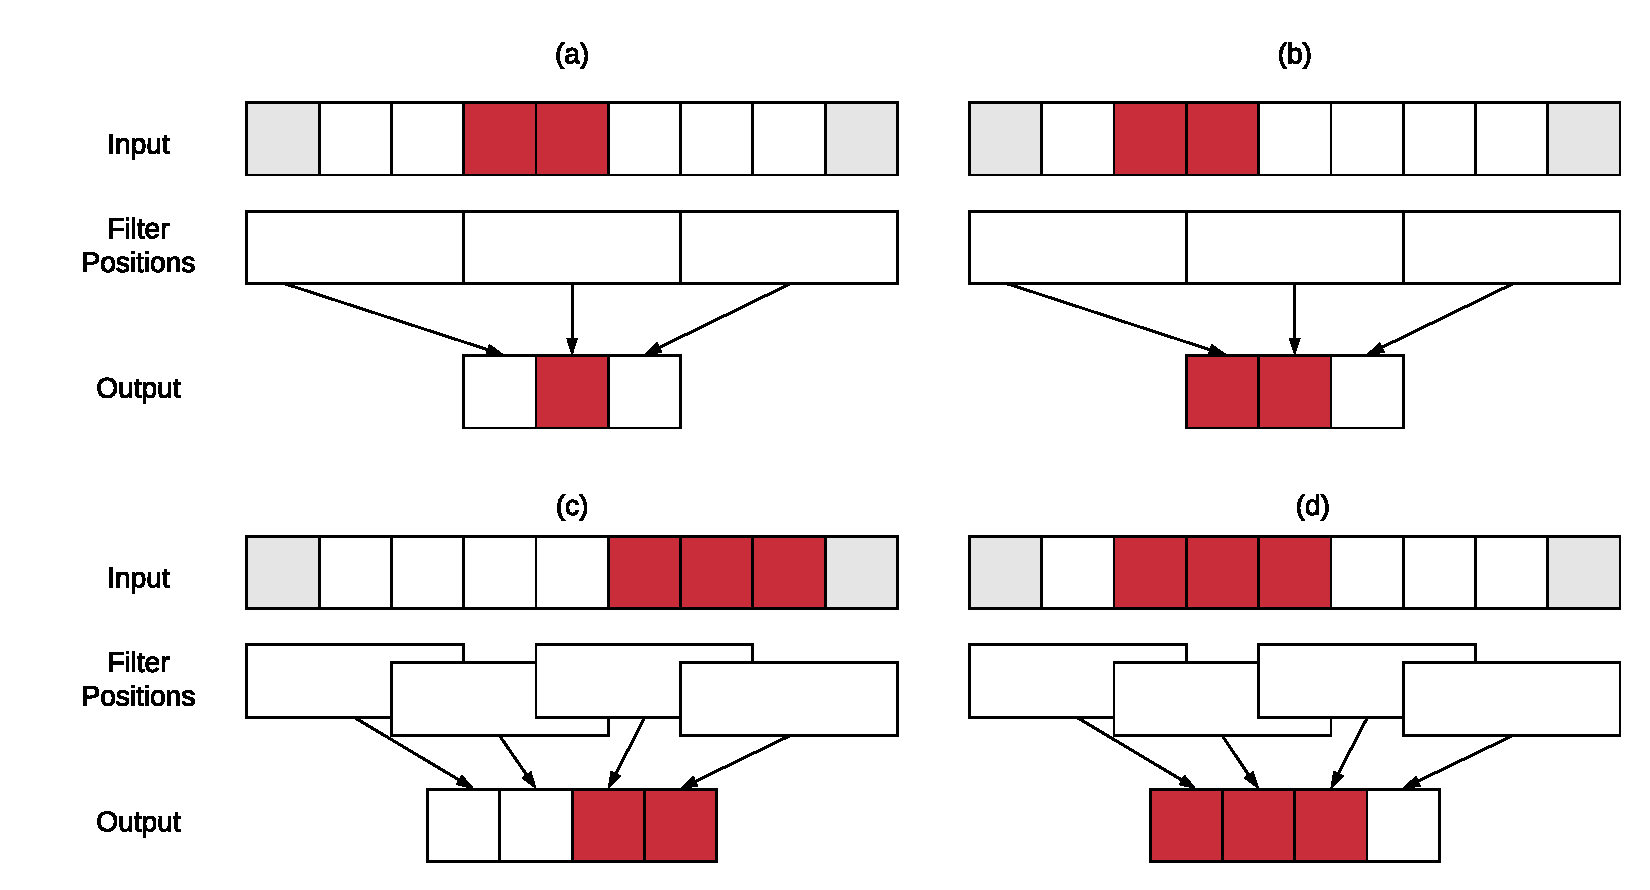
\includegraphics[width=\columnwidth]{images/less_one_example}
\caption{One dimensional representation showing special situations under which actual output size will be smaller than the values calculated by Equations \ref{eqn:xcoordinate} and \ref{eqn:ycoordinate}. (a) and (b) shows a situation with filter stride being equal to the filter size. (c) and (d) shows a situation with input patch being placed at the edge of the input.}
\label{fig:less_one_example}
\end{figure}

It is important to note that there are special situations under which the actual output patch size can be smaller than above calculated value. Consider the simplified one dimensional situation shown in Figure \ref{fig:less_one_example} (a), where the stride value\footnote{Note that the stride value is generally less than or equal to the filter size.} (3) is same as the filter size (3). In this situation the the size of the output patch is one less than the value calculated by Equation \ref{eqn:patchwidth}. However it is not the case in Figure \ref{fig:less_one_example} (b) which has the same input patch size but is placed at a different location. This issue arises only when the stride value is same as the filter size.
Another situation arises when the input patch is placed at the edge of the input as shown in Figure \ref{fig:less_one_example} (c). In this situation it is not possible for the filter to move freely through all filter positions as it hits the input boundary compared to having the input patch on the middle of the input as shown in Figure \ref{fig:less_one_example} (c).
In \system~ we do not distinguish theses differences and use the values calculated by Equation \ref{eqn:patchwidth} and \ref{eqn:patchheight} as they act as an upper bound. In case of a smaller output patch, \system~ simply reads off and updates slightly bigger patches to preserve uniformity.
This also requires updating the starting coordinates of the patches as shown in Equations \ref{eqn:width_subtract} and \ref{eqn:height_subtract}.
Such uniform treatment is required for performing batched inference operations which out of the box gives significant speedups compared to per image inference.

\vspace{2mm}
\hspace{4mm} If $x^O_P + W^O_P > W_{out}:$
\begin{align}
\label{eqn:width_subtract}
x^O_P = &~ W_{out} - W^O_P\\
x^I_P = &~ W_{in} - W^I_P\\
x^R_P = &~ W_{in} - W^R_P
\end{align}

\hspace{4mm} If $y^O_P + H^O_P > H_{out}:$
\begin{align}
\label{eqn:height_subtract}
y^O_P = &~ H_{out} - H^O_P\\
y^I_P = &~ H_{in} - H^I_P\\
y^R_P = &~ H_{in} - H^R_P
\end{align}


\begin{algorithm}
    \caption{Incremental Inference Algorithm}\label{euclid}
    \label{alg:incinference}
    \begin{flushleft}
     \hspace*{4mm} \textbf{Input:} \\
     \hspace*{8mm} $T$ : \textit{Transformation}\\
     \hspace*{8mm} $I$ : \textit{Pre-materialized input from original image}\\
     \hspace*{8mm} $[P^I_1,...,P^I_n]$ : \textit{Input patches}\\
     \hspace*{8mm} $[(x^I_{P_1},y^I_{P_1}),...,(x^I_{P_n},y^I_{P_n})]$ : \textit{Input patch coordinates}\\
     \hspace*{8mm} $W^I_P,H^I_P$ : \textit{Input patch dimensions}
    \end{flushleft}

	\begin{flushleft}
     \hspace*{4mm} \textbf{Output:}\\
     \hspace*{8mm} $[P^O_1,...,P^O_n]$ : \textit{Output patches}\\
     \hspace*{8mm} $[(x^O_{P_1},y^O_{P_1}),...,(x^O_{P_n},y^O_{P_n})]$ : \textit{Output patch coordinates}\\
     \hspace*{8mm} $W^O_P,H^O_P$ : \textit{Output patch dimensions}
    \end{flushleft}

    \begin{algorithmic}[1]
    \Procedure{IncrementalInference}{}
    \State \textit{Calculate} $[(x^O_{P_1},y^O_{P_1}),...,(x^O_{P_n},y^O_{P_n})]$ \textit{and} ($W^O_P,H^O_P$)
    \State \textit{Calculate} $[(x^R_{P_1},y^R_{P_1}),...,(x^R_{P_n},y^R_{P_n})]$ \textit{and} ($W^R_P,H^R_P$)
    \State \textit{Initialize} $R \in \mathcal{\rm I\!R}^{\texttt{depth}(I) \times H^R_P \times W^R_P}$

    \For{\texttt{i in [1,...,n]}}\label{alg:line:memcpy_loop}
    	\State $t_1 \gets I[:,x^R_{P_i}:x^R_{P_i}+W^R_P,y^R_{P_i}:y^R_{P_i}+H^R_P]$ 
    	\State $t_2 \gets P_i \bm\circ_{(x^I_{P_i}-x^R_{P_i}),(y^I_{P_i}-y^R_{P_i})} t_1$
    	\State $R[i,:,:] \gets t_2$
    \EndFor

    \State $[P^O_1,...,P^O_n] \gets T(R)$
    \State \textbf{return} $[P^O_1,...,P^O_n]$, $[(x^O_{P_1},y^O_{P_1}),...,(x^O_{P_n},y^O_{P_n})],$
    \State \hspace*{20mm} ($W^O_P,H^O_P$) 
    \EndProcedure
    \end{algorithmic}

    \vspace*{-2mm}
    \hrulefill
    
    \begin{flushleft}
     \hspace*{4mm} \textbf{Input:}\\
     \hspace*{8mm} $O$ : \textit{Pre-materialized output from original image}\\
     \hspace*{8mm} $[P^O_1,...,P^O_n]$ : \textit{Output patches}\\
     \hspace*{8mm} $[(x^O_{P_1},y^O_{P_1}),...,(x^O_{P_n},y^O_{P_n})]$ : \textit{Output patch coordinates}\\
    \end{flushleft}

    \begin{flushleft}
     \hspace*{4mm} \textbf{Output:}\\
     \hspace*{8mm} $O\textrm'$ : \textit{Updated output}
    \end{flushleft}
	\begin{algorithmic}[1]
    \Procedure{IncrementalToFullProjection}{}
    \State $O\textrm' \gets \texttt{copy}(O)$
    \For{\texttt{i in [1,...,n]}}
    	\State $O\textrm'[i,:,:] \gets P^O_i \bm\circ_{x^O_{P_i},y^O_{P_i}} O\textrm'[i,:,:]$
    \EndFor
    \State \textbf{return} $O\textrm'$
    \EndProcedure

    \end{algorithmic}
\end{algorithm}

With all the geometric mappings defined, we now explain the complete incremental inference approach for a single transformation. Algorithm \ref{alg:incinference} presents it formally.
The \textproc{IncrementalInference} procedure takes in the original transformation $T$, pre-materialized input for $T$ corresponding to original image, a batch of updated patches and their geometric properties as input.
First it calculates geometric properties of the output and read-in patches.
A temporary input volume $R$ is initialized to hold the input patches with their read-in contexts.
The \textsc{for} loop iteratively populates $R$ with corresponding patches.
Finally $T$ is applied on $R$ to compute the output patches.
In a CNN which has multiple such transformations chained together, the outputs of the \textproc{IncrementalInference} procedure are fed as input again for the incremental inference of the next transformation along with the unchanged pre-materialized input corresponding to the new transformation.
However at a local context transformation and global context transformation such as in Conv. $	\rightarrow$ Fully-Connected or Pool $\rightarrow$ Fully-Connected, full updated output has to created as per \textproc{IncrementalToFullProjection} procedure instead of propagating only the updated patches.

\begin{figure}[t]
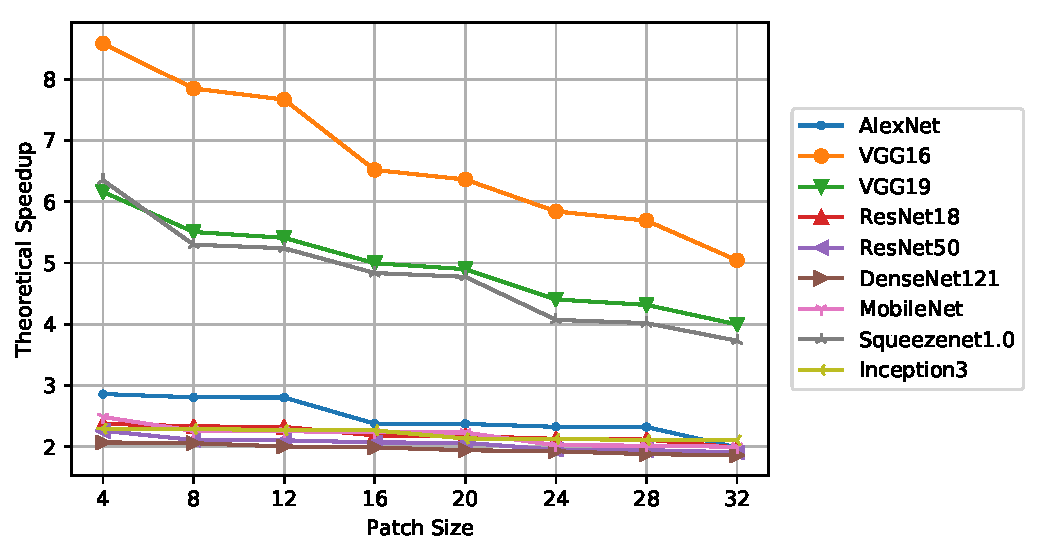
\includegraphics[width=\columnwidth]{images/redundancy_ratio}
\caption{Maximum attainable redundancy ratios of popular CNN architectures when a square occlusion patch of different sizes is placed on the center of the image.}
\label{fig:redundancy_ratio}
\end{figure}

We analyze the maximum attainable redundancy ratios for popular CNN architectures when a square occlusion patch of different sizes is placed on the center\footnote{If the occlusion patch is placed towards to a corner of the input image the redundancy ratio will be slightly higher. But placing the occlusion on the center gives us a worst case estimate.} of the input image. Figure \ref{fig:redundancy_ratio} shows the results. VGG 16-layer version results in the maximum redundancy ratio and Inception V3 model has the lowest redundancy ratio. Most CNN architectures results in a redundancy ratio between 2-3 except VGG 16, VGG 19, and Squeezenet 1.0 CNNs which results in higher redundancy ratios. The attainable redundancy ratio of a CNN is determined by the aspects of it's internal architecture such as number of layers, the size of the filter kernels, and the filter stride values.


\vspace{2mm}
\noindent \textbf{CPU versus GPU implementation considerations.}
Through our experiments we found that even though a straight-forward implementation of \textit{incremental inference} approach as shown in Algorithm \ref{alg:incinference} produces expected speedups for the CPU environment it performs poorly on the GPU environment.
The for loop on the line \ref{alg:line:memcpy_loop} of Algorithm \ref{alg:incinference} is essentially preparing the input for $T$ by copying values from one part of the memory to another sequentially.
This sequential operation becomes a bottleneck for the GPU implementation as it cannot exploit the available parallelism of the GPU effectively.
To overcome this a custom GPU kernel which performs the input preparation more efficiently by parallelly executing the memory copying for each item in the input batch is needed.


\vspace{2mm}
\noindent \textbf{Element-wise addition and depth-wise concatenation.}
Element-wise addition and depth-wise concatenation are two widely used linear algebra operators in CNNs.
Element-wise addition operator requires the two input volumes to have the same dimensions and the depth-wise concatenation requires them to have same spatial dimensions.
Consider a situation for these operators where the first input has incremental spatial update starting at $x^I_{P_1},y^I_{P_1}$ coordinates with dimensions of $H^I_{P_1}$ and $W^I_{P_1}$ and for the second input starting at $x^I_{P_2},y^I_{P_2}$ coordinates with dimensions of $H^I_{P_2}$ and $W^I_{P_2}$.
Then the coordinates and the dimensions of the output and read-in patches can be expressed as follows:

\begin{align}
\label{eqn:laxcoordinate}
x^O_P = x^R_P =&~ min(x^I_{P_1},x^I_{P_2})\\
\label{eqn:laycoordinate}
y^O_P = y^R_P =&~ min(y^I_{P_1},y^I_{P_2})\\
\label{eqn:lapatchwidth}
W^O_P = W^R_P =&~ max(x^I_{P_1}+W^I_{P1},x^I_{P_2}+W^I_{P_2})-min(x^I_{P_1},x^I_{P_2})\\
\label{eqn:lapatchheight}
H^O_P = H^R_P =&~ max(y^I_{P_1}+H^I_{P1},y^I_{P_2}+H^I_{P_2})-min(y^I_{P_1},y^I_{P_2})
\end{align}


\subsection{Projective Field Thresholding}

Projective field \cite{le2017receptive, basiccnnoperations} of a CNN neuron is the local region (including the depth) of the output volume which is connected to it.
The term is borrowed from Neuroscience field where it is used to describe the spatiotemporal effects exerted by a retinal cell on all of the outputs of the neuronal circuitry \cite{de2011projective}.
For our work the notion of projective field is useful as it essentially determines the change propagation path for incremental changes.
The three types of transformations affects the size of the projective field differently. Point transformations does not change of the projective field size while global context transformations increases it to the maximum and local context transformations increase it gradually.
The amount of increase in a local context transformation is determined the filter size and stride parameters. At every transformation the size of the projective field will increase linearly by the filter size and multiplicative by the stride value.

\begin{figure}[t]
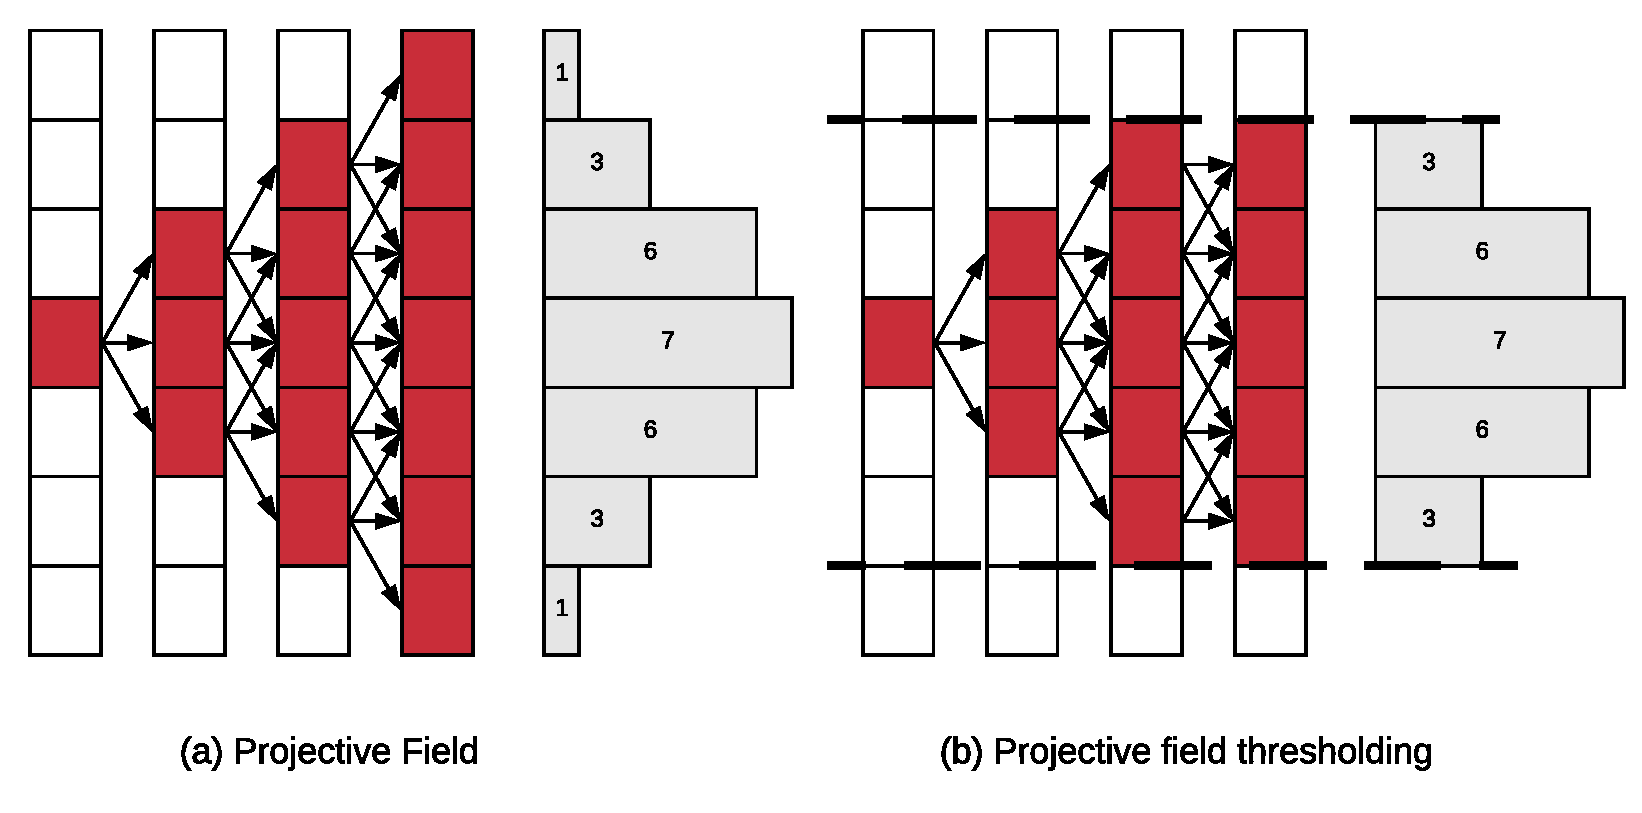
\includegraphics[width=\columnwidth]{images/pf_truncate}
\caption{(a) One dimensional convolution demonstrating projective field growth (filter size = 2, stride = 1). (b) Projective field thresholding with $\tau = 5/7$. Histograms denote the number of unique change propagation paths.}
\label{fig:pf_truncate}
\end{figure}

Because of the projective field growth, even though there will be much computational redundancies in the early layers, towards the latter layers it will decrease or even have no redundancies.
However, we empirically found that the projective field growth can be truncated up to a certain level without significantly affecting the accuracy.
For a more intuitive understanding on why this would work consider the simplified one dimensional convolution example shown in Figure \ref{fig:pf_truncate} (a). In the example a single neuron is modified (marked in red) and a filter of size three is applied with a stride of one repeatedly four times.
Since the filter size is three, each updated neuron will propagate the change to three neurons in the next output layer causing the projective field to grow linearly.
At the end of the fourth layer, the histogram shows the number of unique paths that are available between each output neuron and the original updated neuron in the first layer.
It can be seen that this distribution resembles a Gaussian where many of the paths are connected to the central region.
The amount of actual change in the output layer is determined by both the number of unique paths and also the individual weights of the connections.
But the actual change in the output will converge to a Gaussian in distribution over all possible weight values.
For more details we refer the reader to \cite{luo2016understanding}, where a similar theoretical result has been proved for the receptive field\footnote{Receptive field of a CNN neuron is the local region (including the depth) of the input volume which is connected to it.} of a deep CNN.


As most of the change will be concentrated on the center, we introduce the notion of a projective field threshold $\tau ~ (0 < \tau \leq 1)$ which will be used to restrict the growth of the projective field.
It essentially determines the maximum size of the projective field as a fraction of the size of the input.
Figure \ref{fig:pf_truncate} (b) demonstrates the application of projective field thresholding with a $\tau$ value of $5/7$.
From the histogram generated for the projective field thresholding approach it can be seen that much of the final output change is maintained by this approach while some small changes are lost from the edges.

\begin{figure}[t]
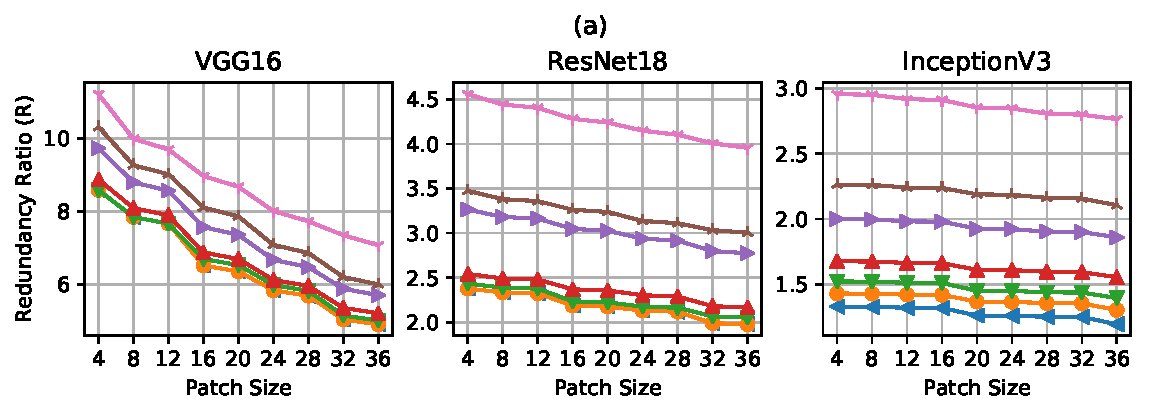
\includegraphics[width=\columnwidth]{images/th_redundancy_ratio}
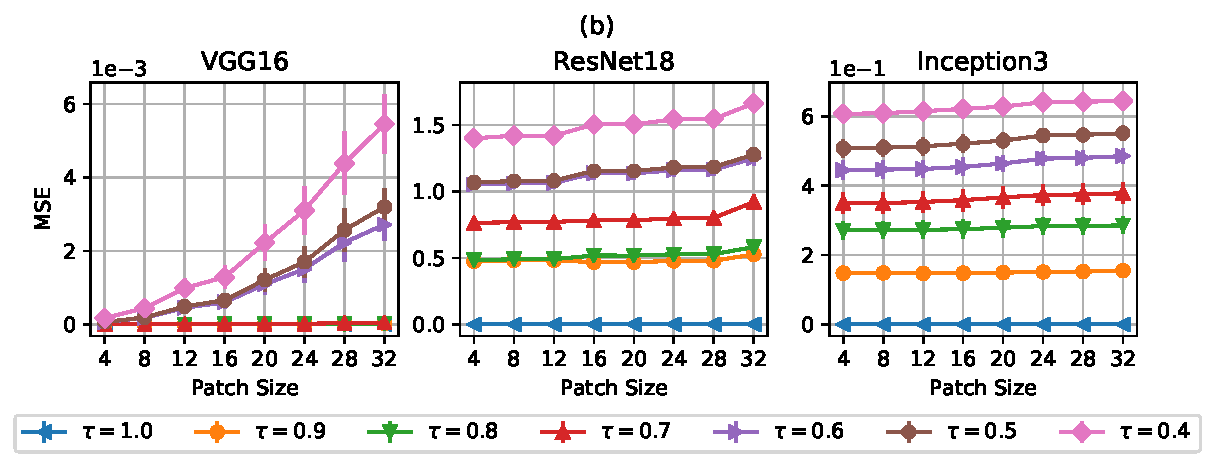
\includegraphics[width=\columnwidth]{images/mse_thresholding}
\caption{(a) Distribution of redundancy ratios for different occlusion patch sizes and projective field thresholding values. (b) Mean Square Error of the final convolution output with different projective field thresholding and occlusion patch sizes for a sample of Diabetic Retinopathy images.}
\label{fig:th_redundancy_ratio}
\end{figure}


\subsection{Adaptive Drill-Down}

\subsection{System Tuning}
